% Appendix Template

\chapter{Registro de respuesta} % Main appendix title

\label{App_Registro} % Change X to a consecutive letter; for referencing this appendix elsewhere, use \ref{AppendixX}

El experimento fue programado de manera tal que los datos obtenidos sobre la ejecución de cada participante se vaciaran en un documento en formato csv, con el título del mismo indicando el número e iniciales del participante, el día en que se este hubiera participado en el experimento y el experimento en que participó.\\

\begin{figure}[th]
\centering
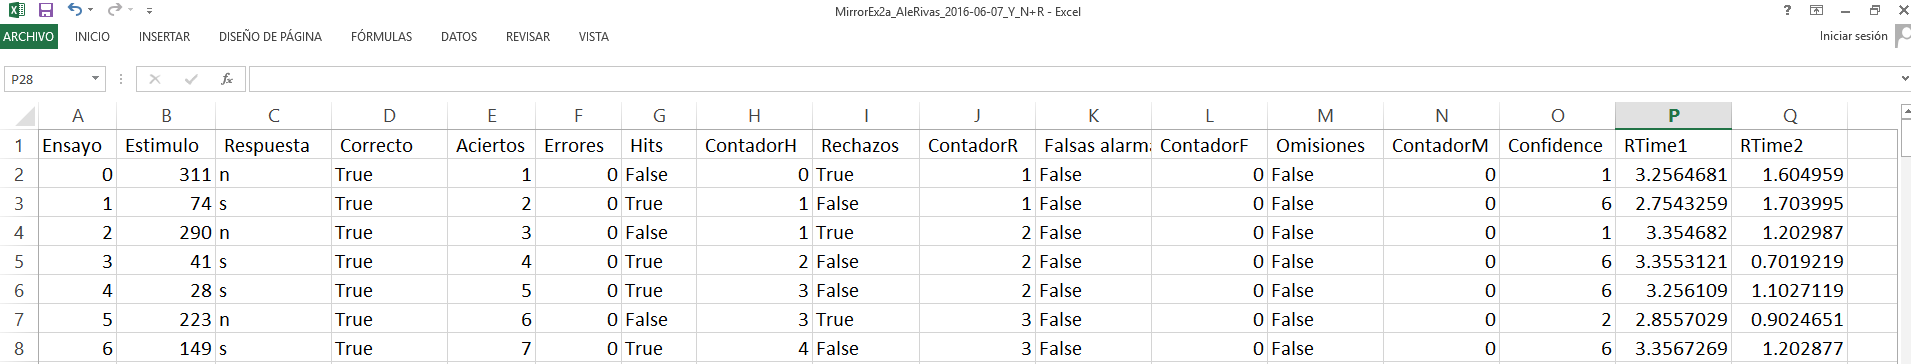
\includegraphics[width=0.95\textwidth]{Figures/csv} 
\decoRule
\caption[Csv muestra]{Captura de pantalla de uno de los archivos csv generados tras la aplicación del experimento. Se ilustra el registro y clasificación de las respuestas emitidas por los participantes en cada ensayo, en función de su correspondencia con el estímulo aleatoriamente mostrado. Se muestran únicamente los primeros seis ensayos del Experimento 2, realizado el 7 de junio del 2016.}
\label{fig:csv}
\end{figure}
\end{itemize}

En la Figura se muestra como ejemplo los primeros seis ensayos registrados en uno de los csv's obtenido tras la realización de nuestro experimento. El csv se fue escribiendo por nuestro programa conforme van avanzando los ensayos, indicándonos cuál de los estímulos diseñados (Estímulo) fue seleccionado aleatoriamente para aparecer en cada ocasión (Ensayo); para señalar el estímulo presentado en cada ensayo se utilizaron números arbitrariamente asignados a cada una de las combinaciones generadas para la elaboración de las figuras de Ebbinghaus (ver las $FIGURAS DE DISEÑO DE ESTIMULOS$). La respuesta del participante se registra (Respuesta) y se clasifica como Correcta o no (se escribe 'True' o 'False' en la columna 'Correcto') de acuerdo a su correspondencia con el estímulo que apareció en pantalla. A continuación, se presentan dos columnas que van registrando la frecuencia acumulada con que el participante acierta y se equivoca a lo largo del experimento (Aciertos y Errores, respectivamente). Además de indicar si se trata de una respuesta acertada, o no, el programa identifica la respuesta emitida por el participante en función a qué tipo de acierto puede ser (Hit o Rechazo) y a qué tipo de error (Falsa alarma u Omision), llevando un contador para cada uno de estos casos que muestra la frecuencia acumulada con que el participante emite una respuesta de cada tipo (ContadorH, para los Hits; ContadorR, para los Rechazos correctos; ContadorF, para las Falsas Alarmas; ContadorM, para las omisiones). En cuanto a la segunda fase de cada ensayo, se registra el puntaje obtenido al aplicar la conversión previamente detallada al número elegido por el participante a la escala de confianza en su respuesta presentada (Confidence). Por último se muestran los Tiempos de Respuesta registrados por cada ensayo: RTime1, corresponde al tiempo de respuesta transcurrido a partir de la aparición del estímulo en pantalla; RTime1b muestra el tiempo transcurrido desde la desaparición del estímulo en pantalla y la emisión de la respuesta del participante; RTime2 presenta el tiempo de respuesta a la segunda fase de cada ensayo.\\ 

